\documentclass[11pt]{article}

\usepackage[a4paper]{geometry}
\geometry{left=2.0cm,right=2.0cm,top=2.5cm,bottom=2.5cm}

\usepackage{ctex} % 支持中文的LaTeX宏包
\usepackage{amsmath,amsfonts,graphicx,subfigure,amssymb,bm,amsthm,mathrsfs,mathtools,breqn} % 数学公式和符号的宏包集合
\usepackage{algorithm,algorithmicx} % 算法和伪代码的宏包
\usepackage[noend]{algpseudocode} % 算法和伪代码的宏包
\usepackage{fancyhdr} % 自定义页眉页脚的宏包
\usepackage[framemethod=TikZ]{mdframed} % 创建带边框的框架的宏包
\usepackage{fontspec} % 字体设置的宏包
\usepackage{adjustbox} % 调整盒子大小的宏包
\usepackage{fontsize} % 设置字体大小的宏包
\usepackage{tikz,xcolor} % 绘制图形和使用颜色的宏包
\usepackage{multicol} % 多栏排版的宏包
\usepackage{multirow} % 表格中合并单元格的宏包
\usepackage{pdfpages} % 插入PDF文件的宏包
\RequirePackage{listings} % 在文档中插入源代码的宏包
\RequirePackage{xcolor} % 定义和使用颜色的宏包
\usepackage{wrapfig} % 文字绕排图片的宏包
\usepackage{bigstrut,multirow,rotating} % 支持在表格中使用特殊命令的宏包
\usepackage{booktabs} % 创建美观的表格的宏包
\usepackage{circuitikz} % 绘制电路图的宏包

\definecolor{dkgreen}{rgb}{0,0.6,0}
\definecolor{gray}{rgb}{0.5,0.5,0.5}
\definecolor{mauve}{rgb}{0.58,0,0.82}
\lstset{
  frame=tb,
  aboveskip=3mm,
  belowskip=3mm,
  showstringspaces=false,
  columns=flexible,
  framerule=1pt,
  rulecolor=\color{gray!35},
  backgroundcolor=\color{gray!5},
  basicstyle={\small\ttfamily},
  numbers=none,
  numberstyle=\tiny\color{gray},
  keywordstyle=\color{blue},
  commentstyle=\color{dkgreen},
  stringstyle=\color{mauve},
  breaklines=true,
  breakatwhitespace=true,
  tabsize=3,
}

% 轻松引用, 可以用\cref{}指令直接引用, 自动加前缀. 
% 例: 图片label为fig:1
% \cref{fig:1} => Figure.1
% \ref{fig:1}  => 1
\usepackage[capitalize]{cleveref}
% \crefname{section}{Sec.}{Secs.}
\Crefname{section}{Section}{Sections}
\Crefname{table}{Table}{Tables}
\crefname{table}{Table.}{Tabs.}

\setmainfont{Palatino_Linotype}[
  Path = ../Fonts/,
  Extension = .ttf
]
\setCJKmainfont{SimHei}[
  Path = ../Fonts/,
  Extension = .ttf
]
\punctstyle{kaiming}
% 偏好的几个字体, 可以根据需要自行加入字体ttf文件并调用

\renewcommand{\emph}[1]{\begin{kaishu}#1\end{kaishu}}

%改这里可以修改实验报告表头的信息
\newcommand{\studentNum}{00000000}
\newcommand{\name}{我是谁}
\newcommand{\exDate}{2025.03.18}
\newcommand{\weekDay}{二}
\newcommand{\ap}{下午}
%%%%%%%%%%%%%%%%%%%%%%%%%%%

\begin{document}

%若需在页眉部分加入内容, 可以在这里输入
% \pagestyle{fancy}
% \lhead{\kaishu 测试}
% \chead{}
% \rhead{}

\begin{center}
    \LARGE \bf 《\, 基\, 础\, 物\, 理\, 实\, 验\, 》\, 实\, 验\, 报\, 告
\end{center}

\begin{center}
    \emph{学号}\underline{\makebox[6em][c]{\studentNum}}
    \emph{姓名}\underline{\makebox[6em][c]{\name}} 
    \emph{实验日期} \underline{\makebox[8em][c]{\exDate}}
    \emph{星期} \underline{\makebox[2em][c]{\weekDay}}\;\underline{\makebox[3em][c]{\ap}}
    {\noindent}
    \rule[8pt]{17cm}{0.2em}
\end{center}

\begin{center}
    \Large \bf 脉搏、语音及图像信号的傅里叶分析
\end{center}

\section*{一、实验目的}

\begin{enumerate}
    \item 了解常用周期信号的傅里叶级数表示。
    \item 了解周期脉搏信号、语音信号及图像信号的傅里叶分析过程。
    \item 理解体会傅里叶分析的理论及现实意义。
\end{enumerate}

\section*{二、实验仪器}

脉搏语音实验仪器,数字信号发生器,信号加法器,电脑。

\section*{三、实验原理}

\begin{enumerate}
    \item 任意一个周期为$T$的周期信号$f(t)$都可以表示为傅里叶级数:
    \begin{align*}
        f(t) &= \frac{1}{2}a_0 + \sum_{n=1}^{\infty}(a_n \cos n\omega_0 t + b_n \sin n\omega_0 t)\\
        a_0 &= \frac{1}{\pi}\int_{-\pi}^{\pi}f(\omega_0t)d(\omega_0t)\\
        a_n &= \frac{1}{\pi}\int_{-\pi}^{\pi}f(\omega_0t)\cos(n\omega_0t)d(\omega_0t)\\
        b_n &= \frac{1}{\pi}\int_{-\pi}^{\pi}f(\omega_0t)\sin(n\omega_0t)d(\omega_0t)
    \end{align*}
    其中,其中$\omega_0$为角频率,称为基频,$a_0$为常数,$a_n$和$b_n$称为第$n$次谐波的幅值。任何周期性非简谐交变信号均可用上述傅里叶级数进行展开,即分解为一系列不同次谐波的叠加。
    \item 方波在一个周期内的函数表达式为:
    $$
    f(t)=\left\{
        \begin{array}{cc}
        h & 0\leq t<\frac{T}{2} \\
        -h & -\frac{T}{2}\leq t<0
        \end{array}
        \right.
    $$
    其傅里叶级数展开为:
    \begin{align*}
        f(t)&=\dfrac{4h}{\pi}\sum_{n=1}^{\infty}\dfrac{1}{2n-1}\sin(2n-1)\omega_0t\\
        &=\dfrac{4h}{\pi}\left(\sin\omega_0t+\dfrac{1}{3}\sin3\omega_0t+\dfrac{1}{5}\sin5\omega_0t+\cdots\right)
    \end{align*}
    三角波的函数表达式为:
    $$
    f(t)=\left\{
        \begin{array}{cc}
        \dfrac{4h}{T}t & -\frac{T}{4}\leq t<\frac{T}{4} \\
        2h(1-\dfrac{2t}{T}) & \frac{T}{4}\leq t<\frac{3T}{4}
        \end{array}
        \right.
    $$
    其傅里叶级数展开为:
    \begin{align*}
        f(t)&=\dfrac{4h}{\pi^2}\sum_{n=1}^{\infty}(-1)^{n-1}\dfrac{1}{(2n-1)^2}\sin(2n-1)\omega_0t\\
        &=\dfrac{8h}{\pi^2}\left(\sin\omega_0t-\dfrac{1}{3^2}\sin3\omega_0t+\dfrac{1}{5^2}\sin5\omega_0t+\cdots\right)
    \end{align*}
    从以上各式可知,任何周期信号都可以表示为无限多次谐波的叠加,谐波次数越高,振幅越小,它对叠加波的贡献就越小,当小至一定程度时(谐波振幅小于基波振幅的$5\%$),则高次的谐波就可以忽略而变成有限次数谐波的叠加,这对设计仪器电路是很有意义的。
\end{enumerate}

\section*{四、实验内容}

\begin{enumerate}
    \item 傅里叶级数的合成
    
    \begin{center}
        \Large{标准信号/外接}
    \end{center}
    
    \begin{enumerate}
        \item 利用数字信号发生器产生频率分别为$100\,Hz$、$300\,Hz$、$500\,Hz$的正弦波信号,并使其位相相同,振幅比为$1:\dfrac{1}{3}:\dfrac{1}{5}$,将上述三个信号,分别通过加法器输入到傅里叶分析仪,观察和记录波形。
        \begin{figure}[H]
            \centering
            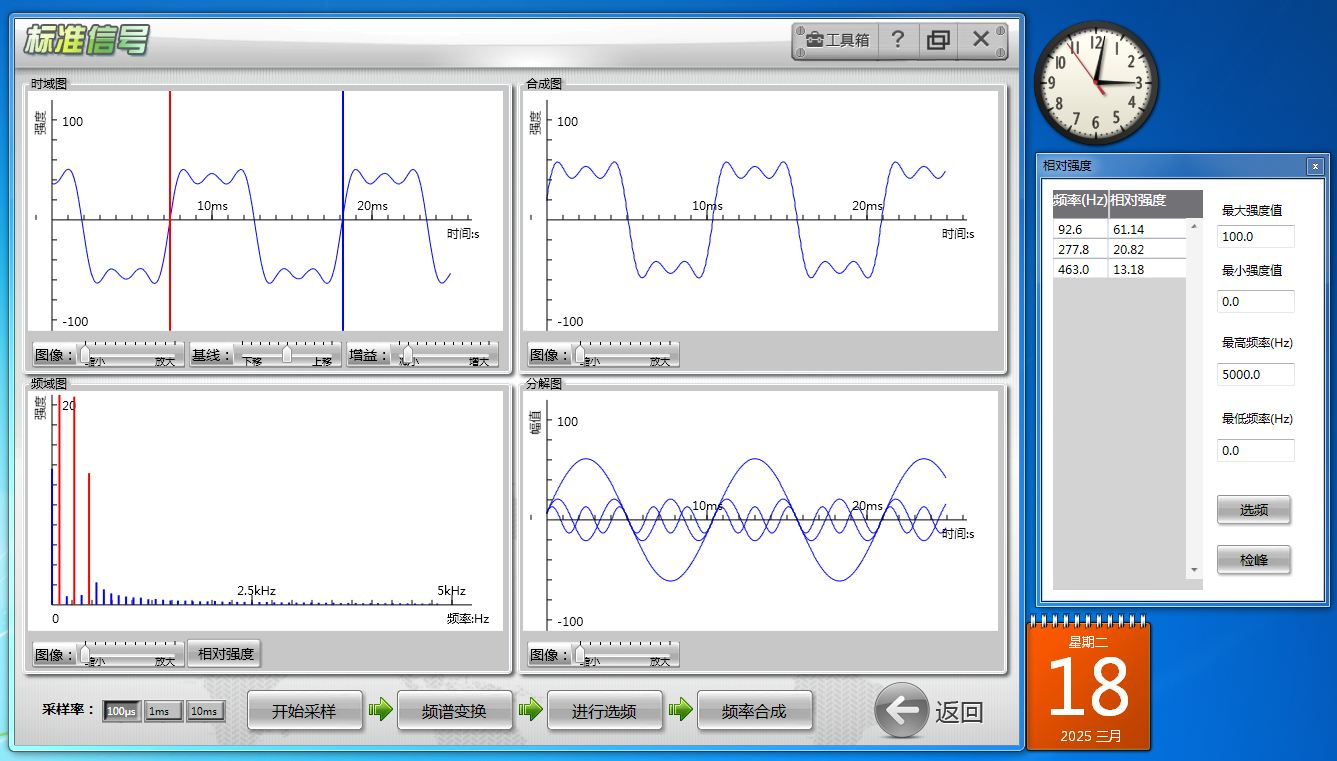
\includegraphics[width=15cm]{Fig/图1 信号发生器合成方波.JPG}
            \caption{信号发生器合成方波}
        \end{figure}
        \item 利用数字信号发生器产生方波,输入到傅里叶分析仪,并将其与上述合成后的信号相比较。
        \begin{figure}[H]
            \centering
            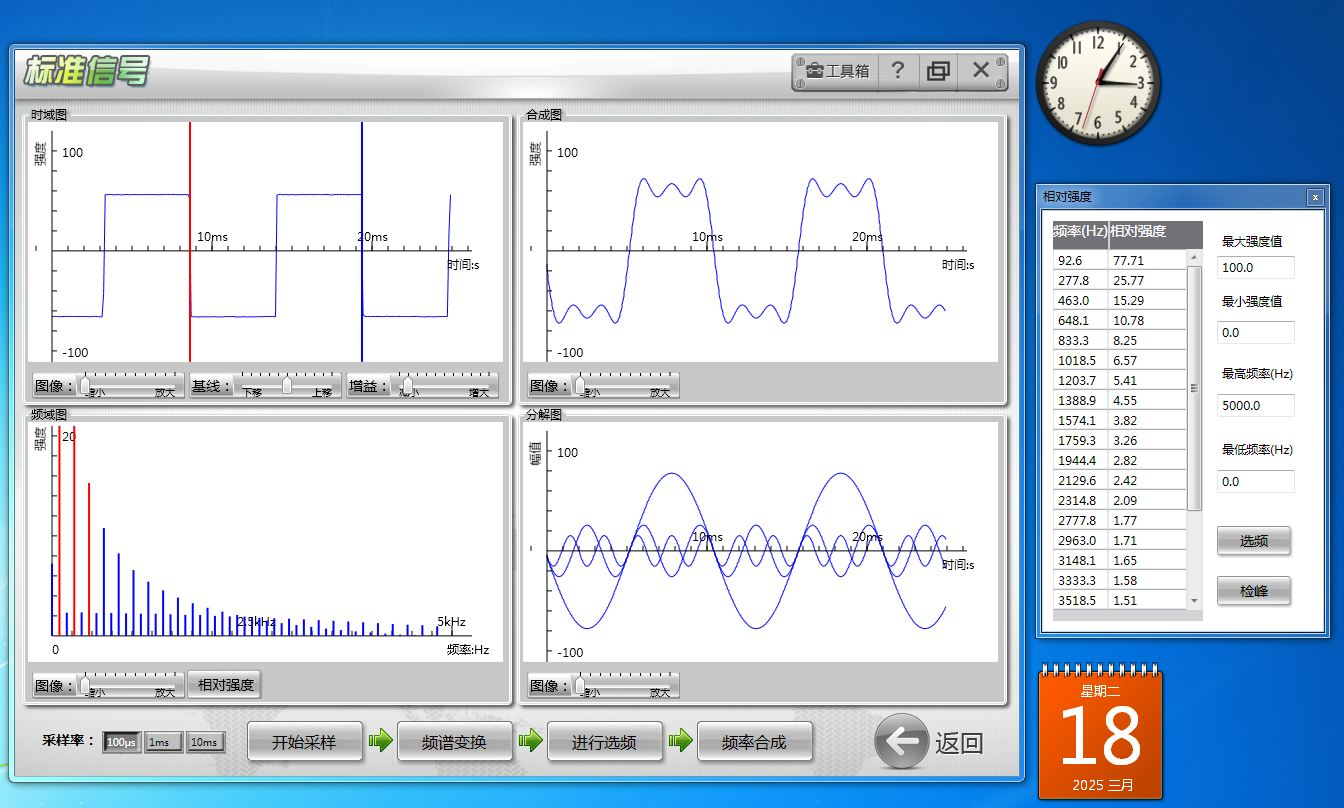
\includegraphics[width=15cm]{Fig/图2 信号发生器输出方波.JPG}
            \caption{信号发生器输出方波}
        \end{figure}
        \item 利用数字信号发生器产生频率分别为$200\,Hz$、$600\,Hz$、$1000\,Hz$的正弦信号,振幅比为$1:\dfrac{1}{3^2}:\dfrac{1}{5^2}$,并且保证其相位相差$180^\circ$,然后通过加法器输入到傅里叶分析仪,观察并记录其波形,并与数字信号发生器产生的三角波相比较。
        \begin{figure}[H]
            \centering
            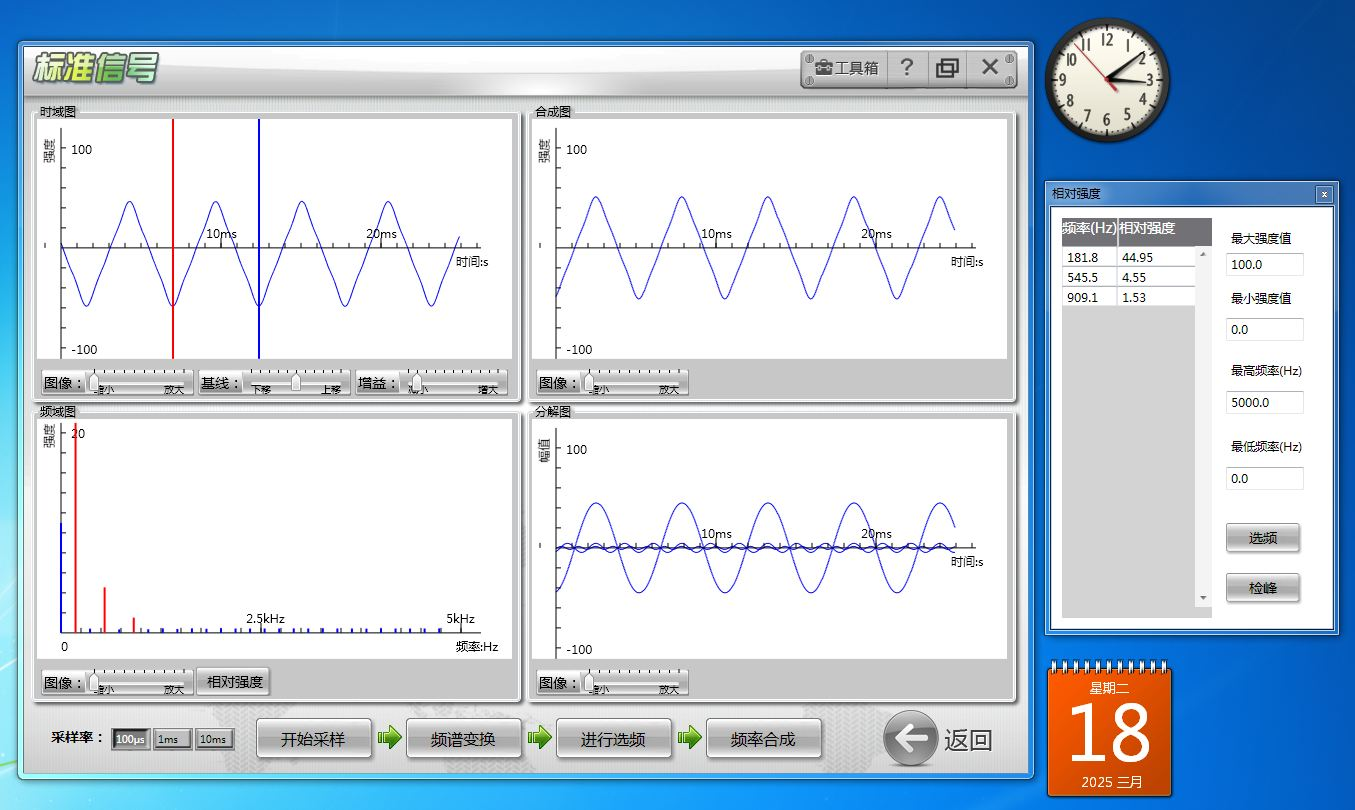
\includegraphics[width=15cm]{Fig/图3 信号发生器合成三角波.JPG}
            \caption{信号发生器合成三角波}
        \end{figure}
        \begin{figure}[H]
            \centering
            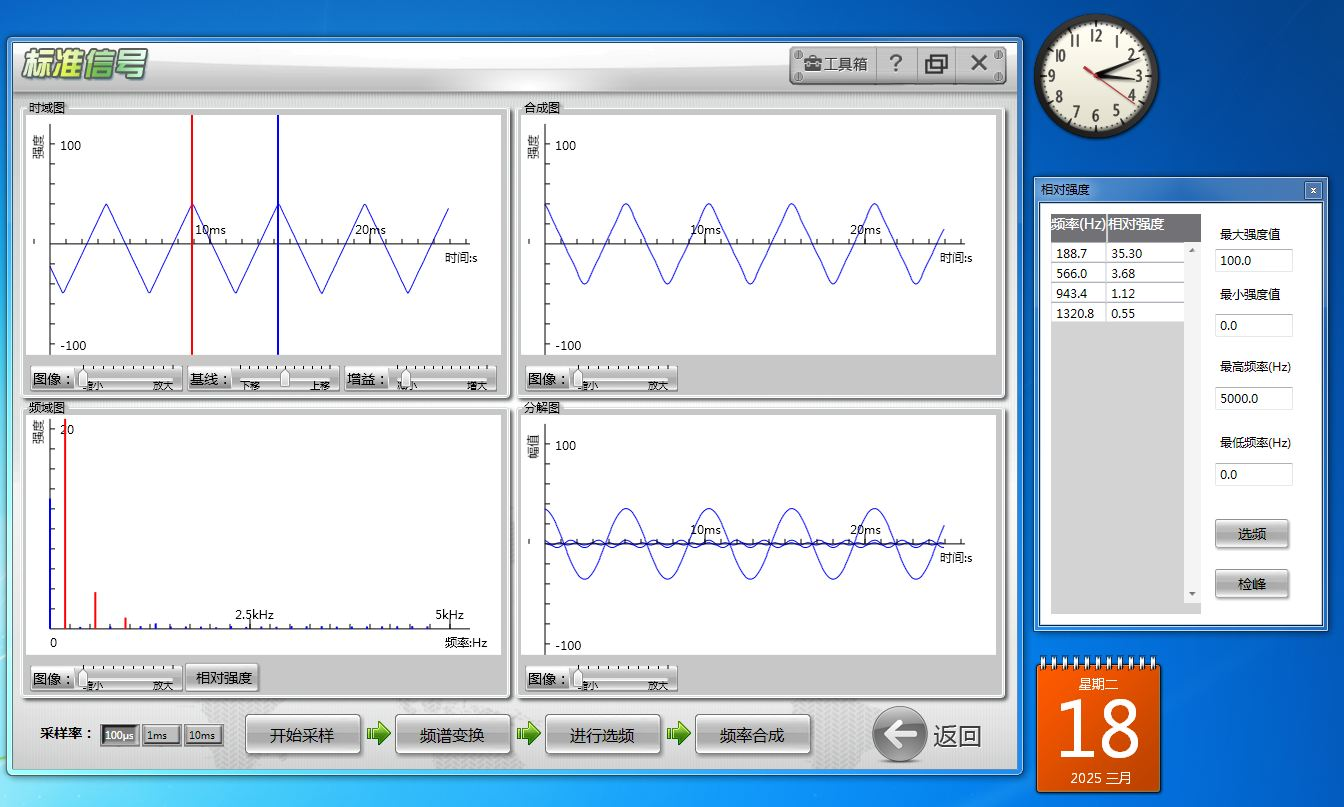
\includegraphics[width=15cm]{Fig/图4 信号发生器输出三角波.JPG}
            \caption{信号发生器输出三角波}
        \end{figure}
    \end{enumerate}
    
    \begin{center}
        \Large{标准信号/内接}
    \end{center}
    
    利用傅里叶分析仪分别产生方波与三角波,进行傅里叶分析,记录各正弦波频率以及相对的幅度之间的关系,并与上述加法器输入信号相比较。

    滤波与选频分析:对上述傅里叶分析的频谱,分别选择低频段和高频段信号通
    过傅里叶反变换,观察它们图像并导出保存,试分析低通滤波和高通滤波图像的区别。

    \begin{figure}[H]
        \centering
        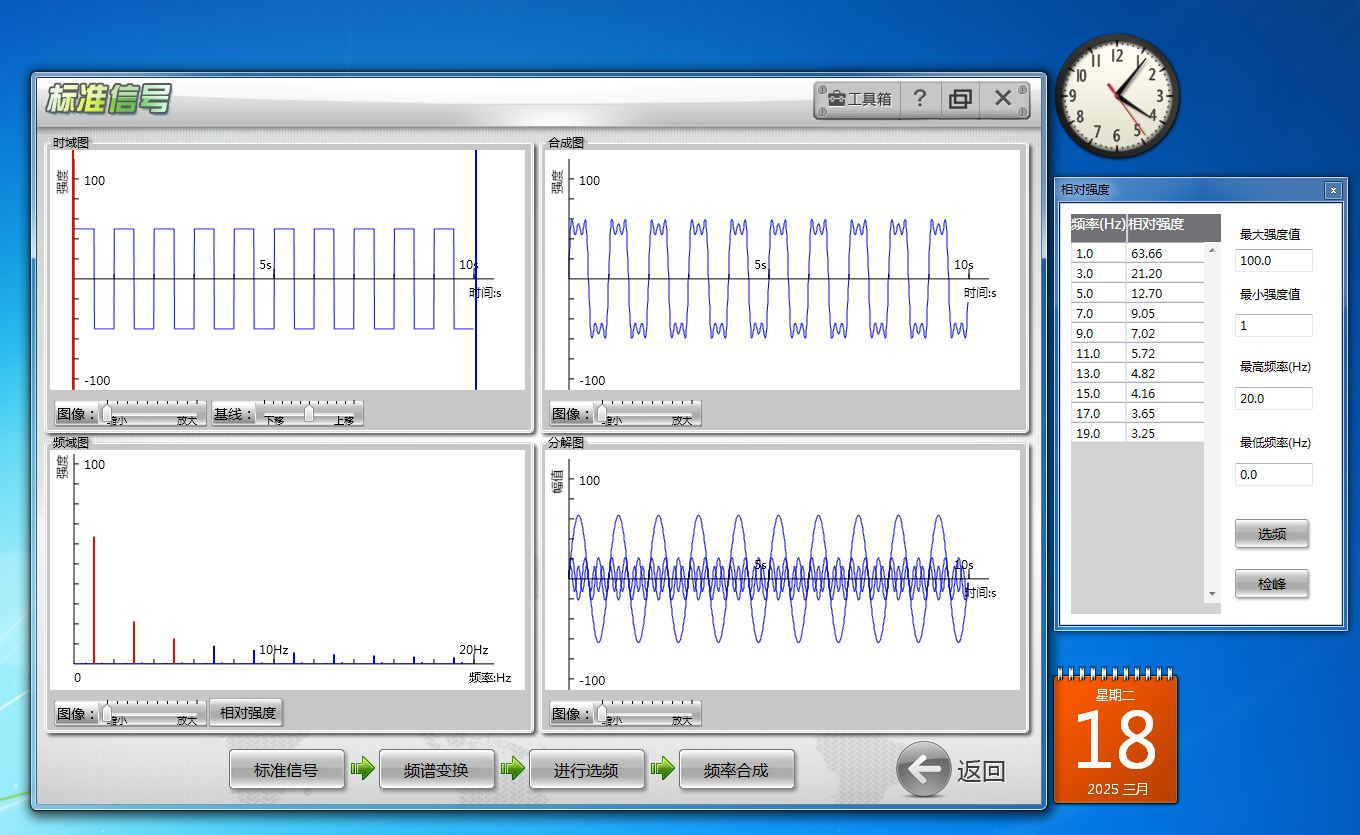
\includegraphics[width=15cm]{Fig/图5 内置方波信号的分解和低通滤波.JPG}
        \caption{内置方波信号的分解和低通滤波}
    \end{figure}
    \begin{figure}[H]
        \centering
        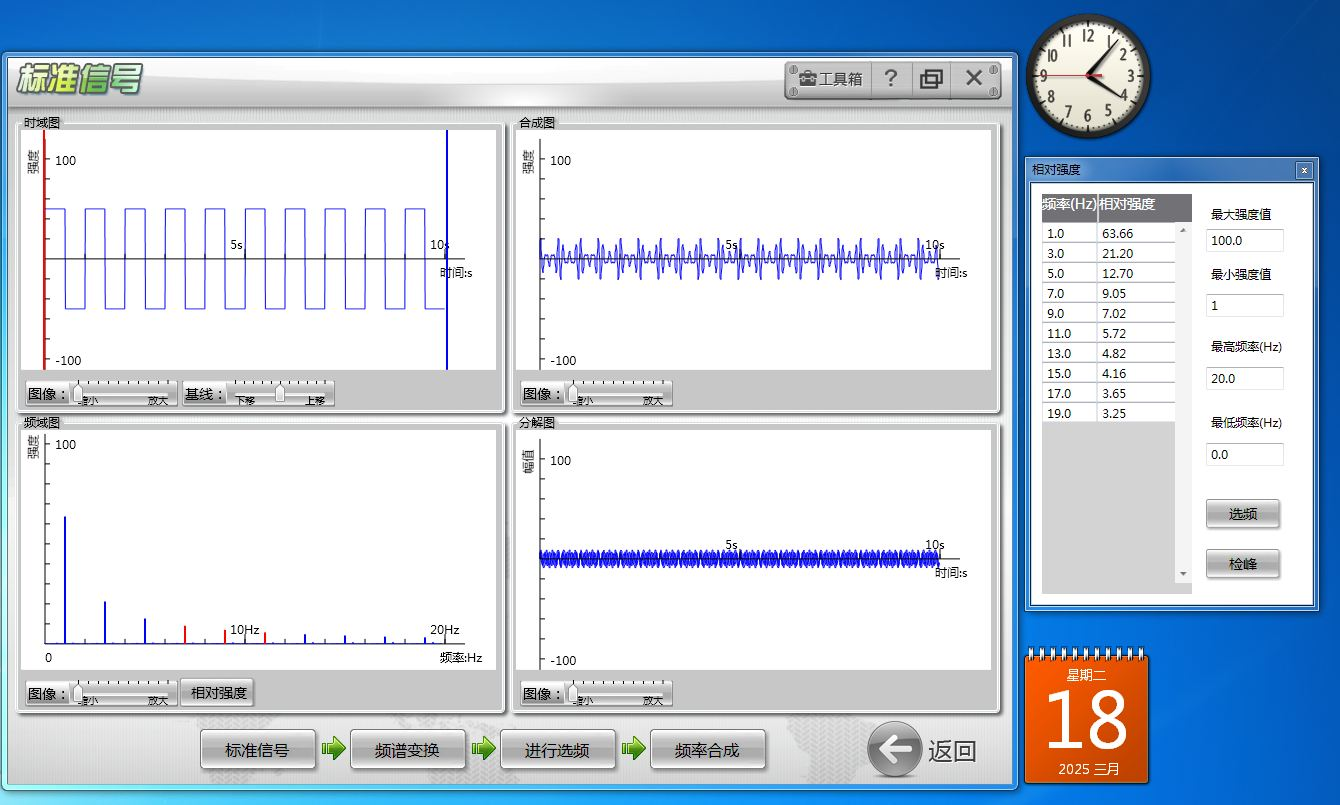
\includegraphics[width=15cm]{Fig/图6 内置方波信号的分解和高通滤波.JPG}
        \caption{内置方波信号的分解和高通滤波}
    \end{figure}
    \begin{figure}[H]
        \centering
        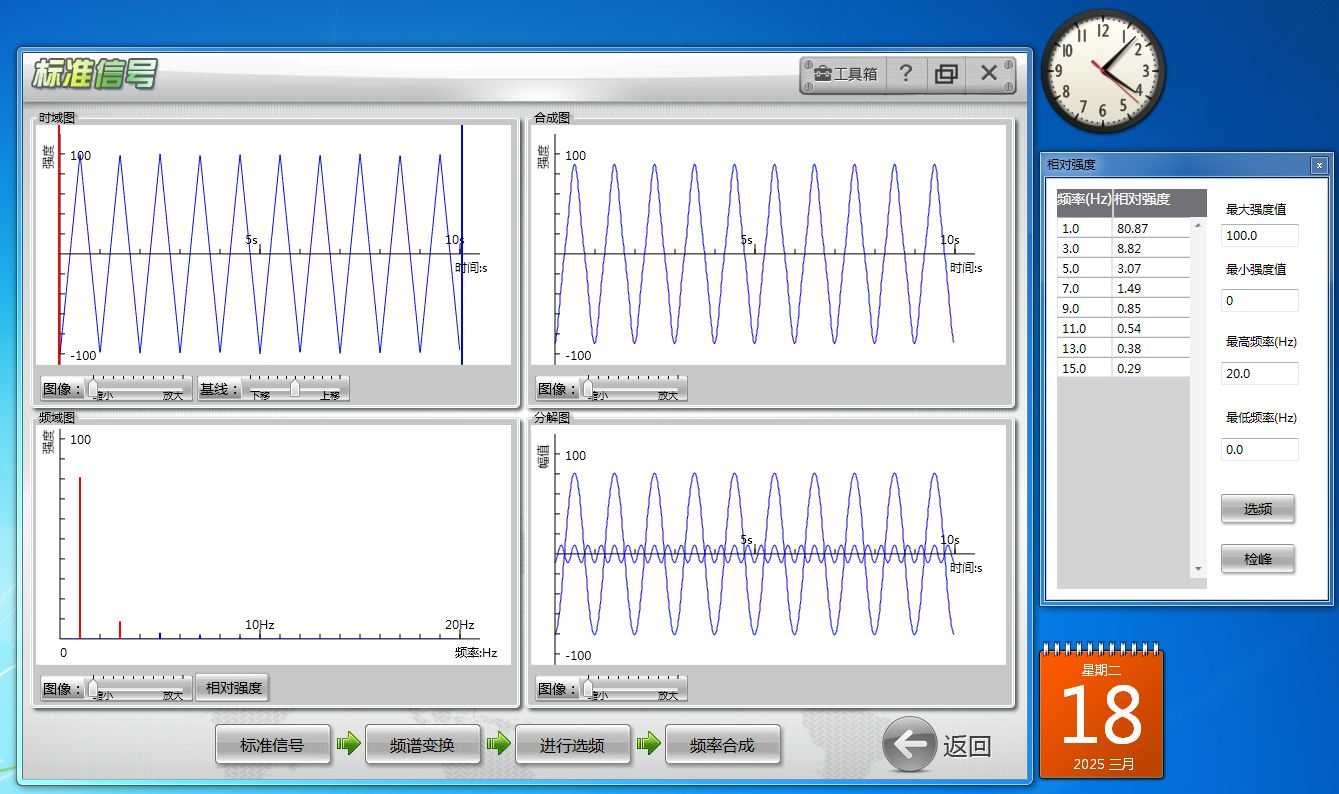
\includegraphics[width=15cm]{Fig/图7 内置三角波信号的分解和低通滤波.JPG}
        \caption{内置三角波信号的分解和低通滤波}
    \end{figure}
    \begin{figure}[H]
        \centering
        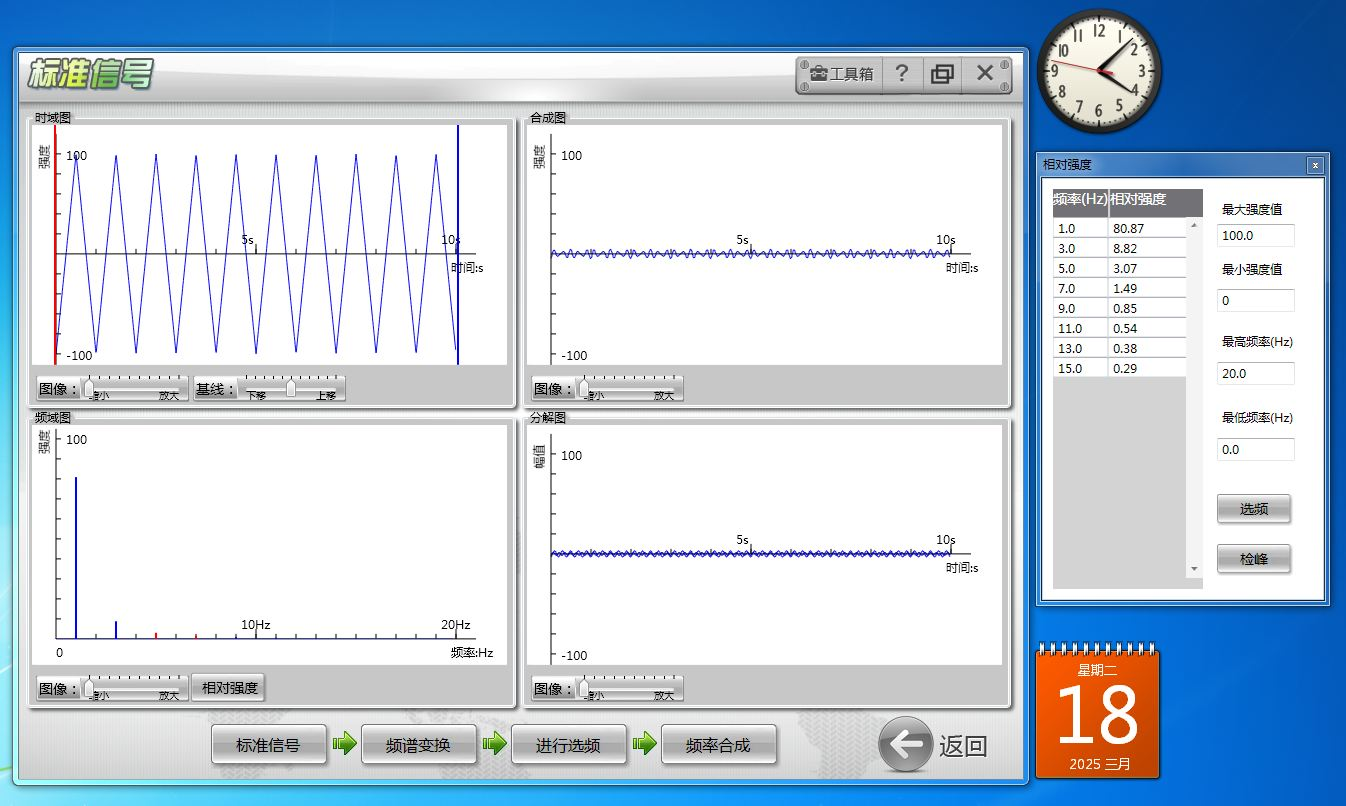
\includegraphics[width=15cm]{Fig/图8 内置三角波信号的分解和高通滤波.JPG}
        \caption{内置三角波信号的分解和高通滤波}
    \end{figure}

    \item “脉搏信号”的傅里叶分析
    \begin{enumerate}
        \item 用傅里叶分析仪软件中提供的“脉搏信号”模块和脉搏语音仪上的光电探测器测试自己脉搏波的信号,观察你的脉搏信号。
        \item 选择完整的周期信号进行频谱分析,并选择合适的频段,测量其中心频率。
        \begin{figure}[H]
            \centering
            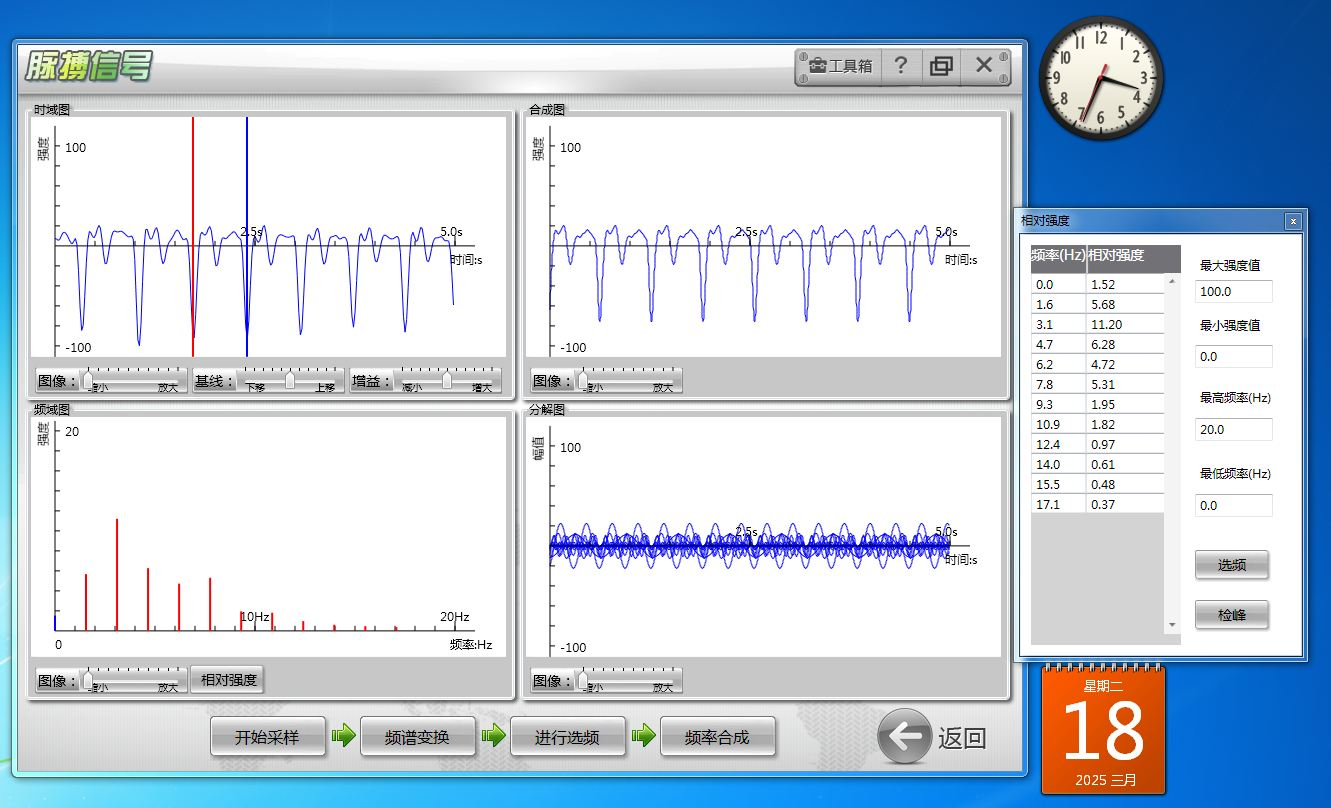
\includegraphics[width=15cm]{Fig/图9 脉搏信号.JPG}
            \caption{脉搏信号}
        \end{figure}
        \item 深呼吸后,重复上述实验,请比较两次中心频率的变化。
        \begin{figure}[H]
            \centering
            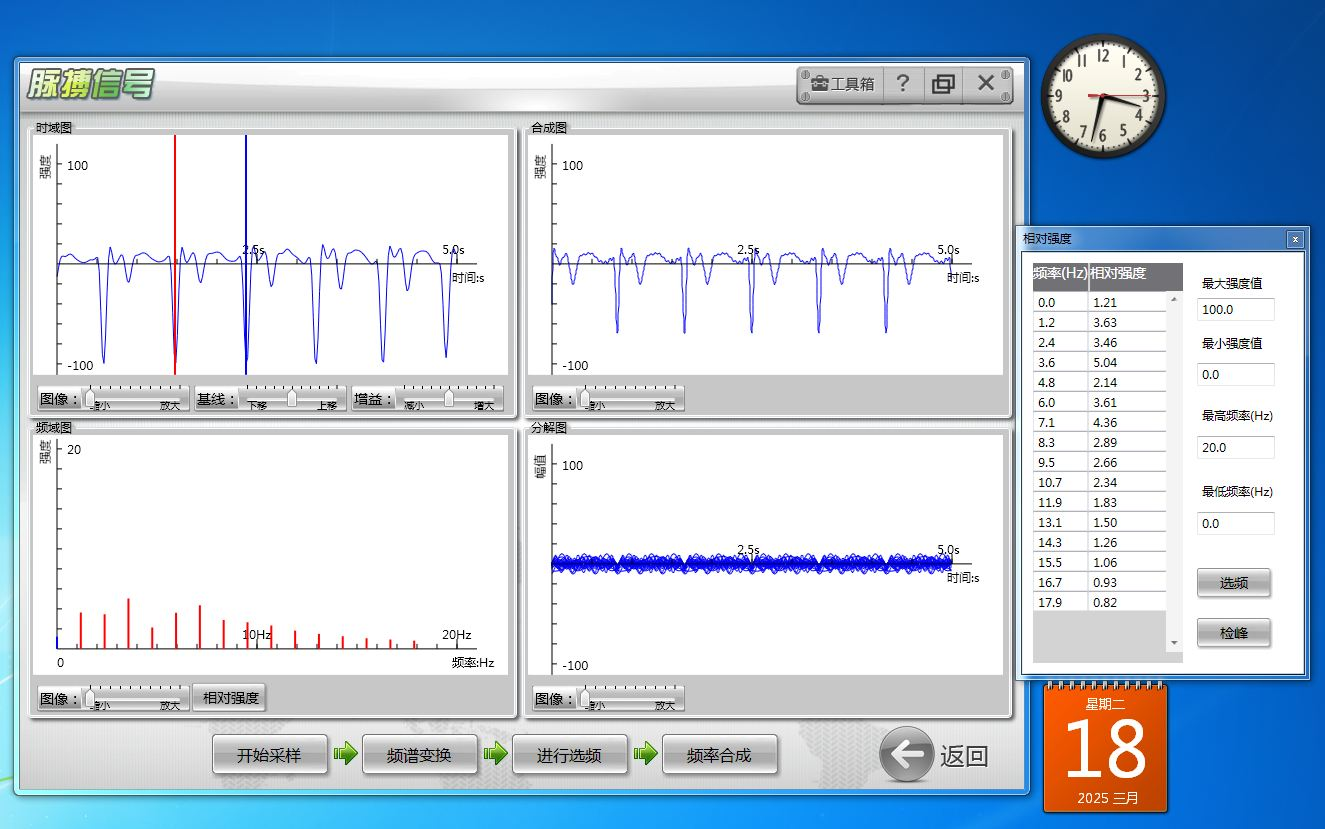
\includegraphics[width=15cm]{Fig/图10 深呼吸后的脉搏信号.JPG}
            \caption{深呼吸后的脉搏信号}
        \end{figure}
    \end{enumerate}

    \item 语音信号的傅里叶分析与识别
    \begin{enumerate}
        \item 用傅里叶分析仪软件提供的“语音信号”模块,通过外置麦克风采集语音信号,并选择合适的频段,记录该频段语音信号的傅里叶分析频谱。
        \begin{figure}[H]
            \centering
            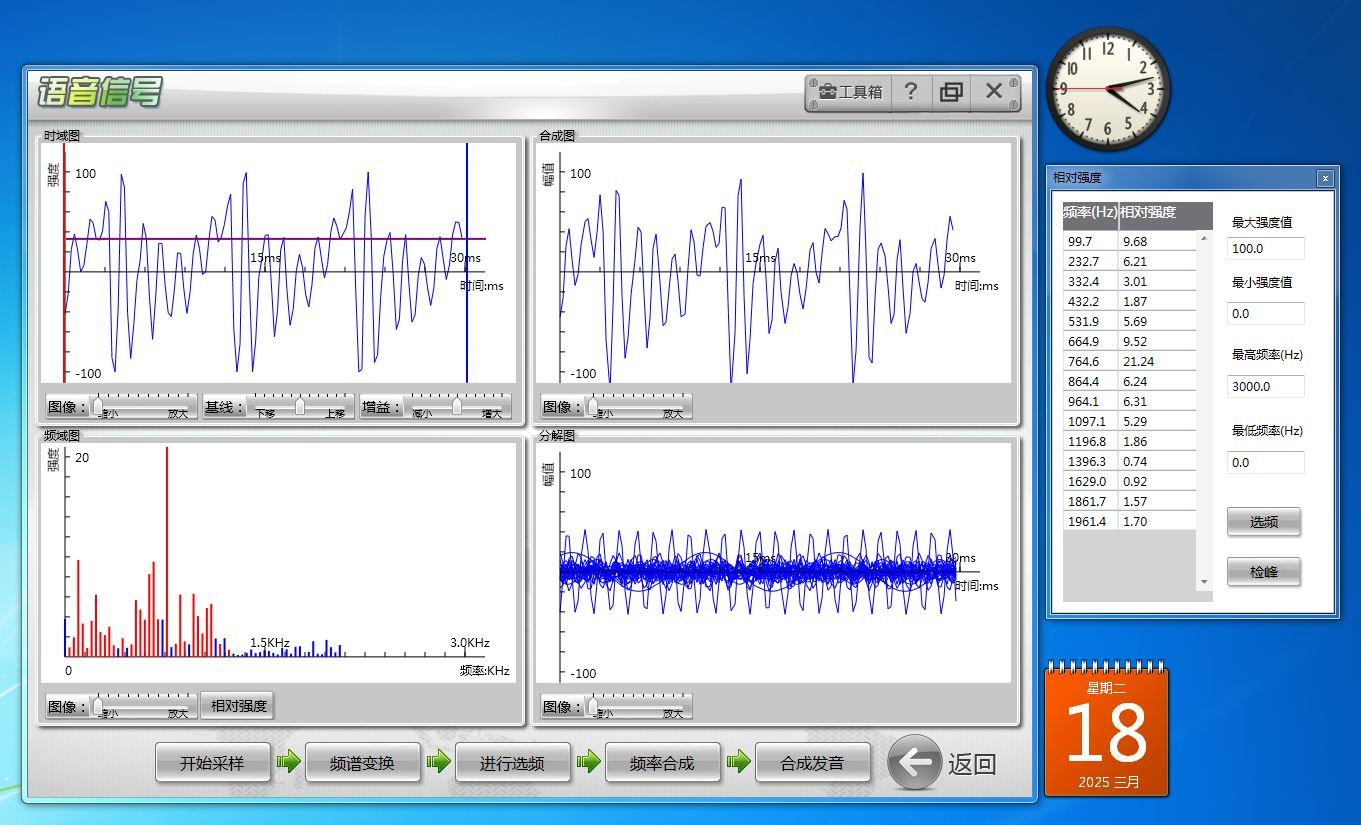
\includegraphics[width=15cm]{Fig/图11 语音信号.JPG}
            \caption{语音信号}
        \end{figure}
        \item 语音对比
        
        利用软件提供的“语音对比”模块,通过麦克风采集两次相同或不同元音的信号,重复上述过程,分别记录两次频谱的分布,体验语音识别功能。

        完成“a”音的通道A信号采集,频谱变化;通道B信号采集,频谱变换;语音识别和谱线对比。
        \begin{figure}[H]
            \centering
            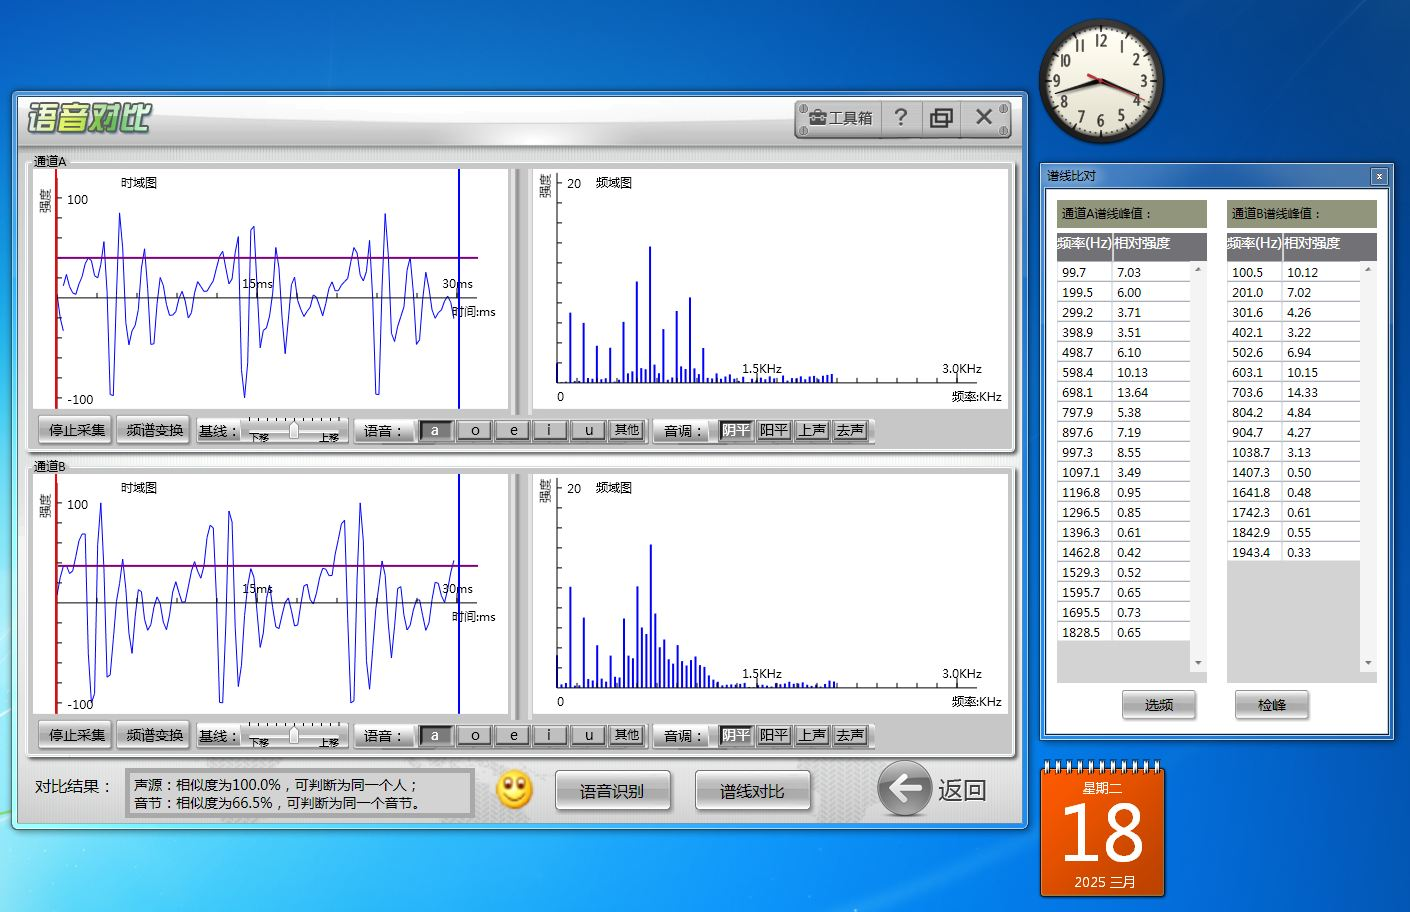
\includegraphics[width=15cm]{Fig/图12 语音a的识别.JPG}
            \caption{语音a的识别}
        \end{figure}
        完成“i”音的通道A信号采集,频谱变化;通道B信号采集,频谱变换;语音识别和谱线对比
        \begin{figure}[H]
            \centering
            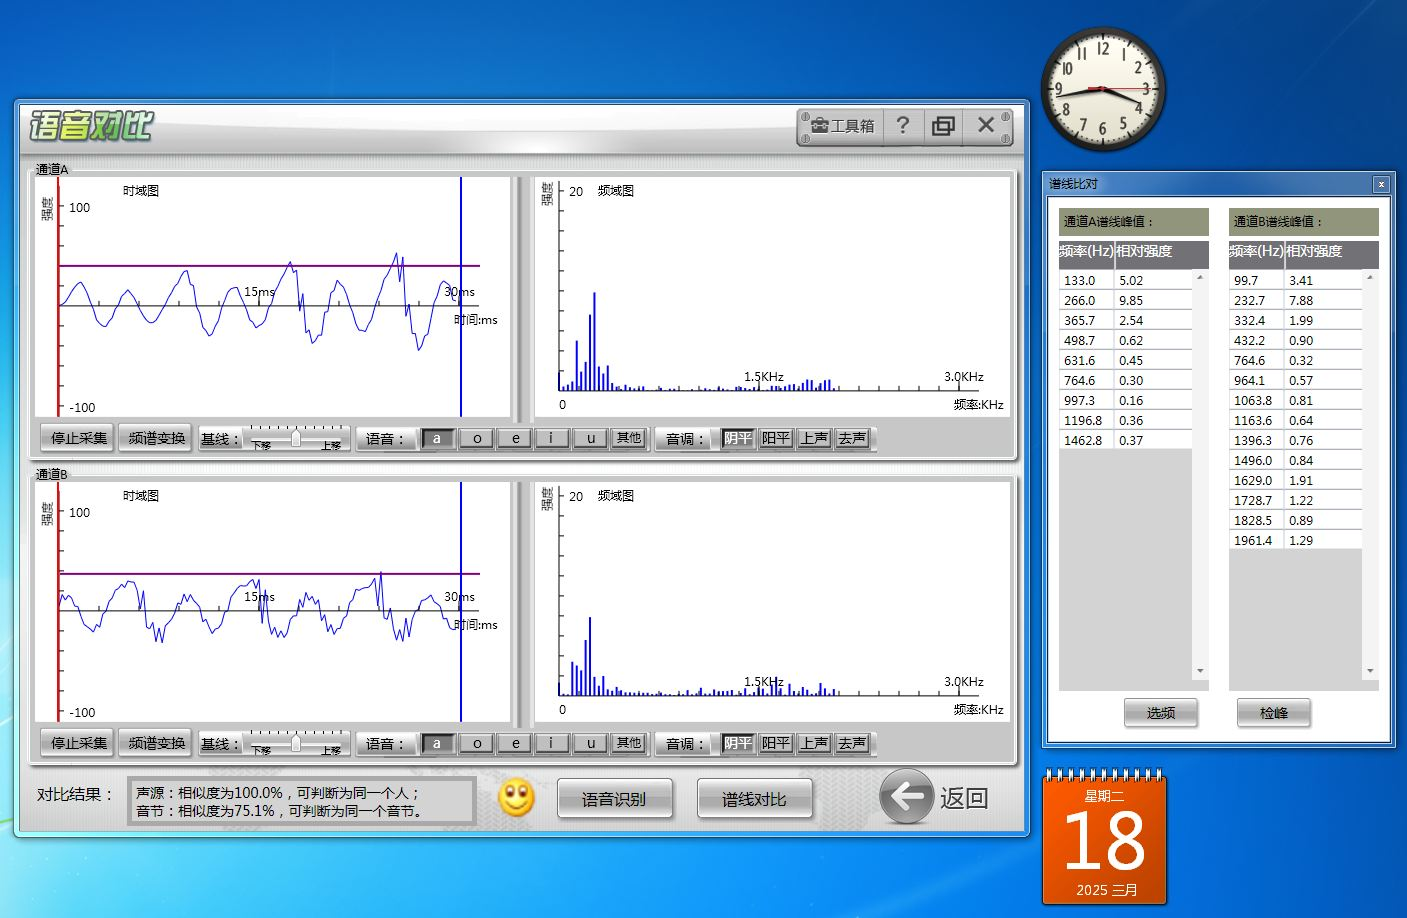
\includegraphics[width=15cm]{Fig/图13 语音i的识别.JPG}
            \caption{语音i的识别}
        \end{figure}
        \item “长时语音”
        
        通过外置麦克风采集一段语音信号,并观察傅里叶分析频谱实时频谱变化。
        \begin{figure}[H]
            \centering
            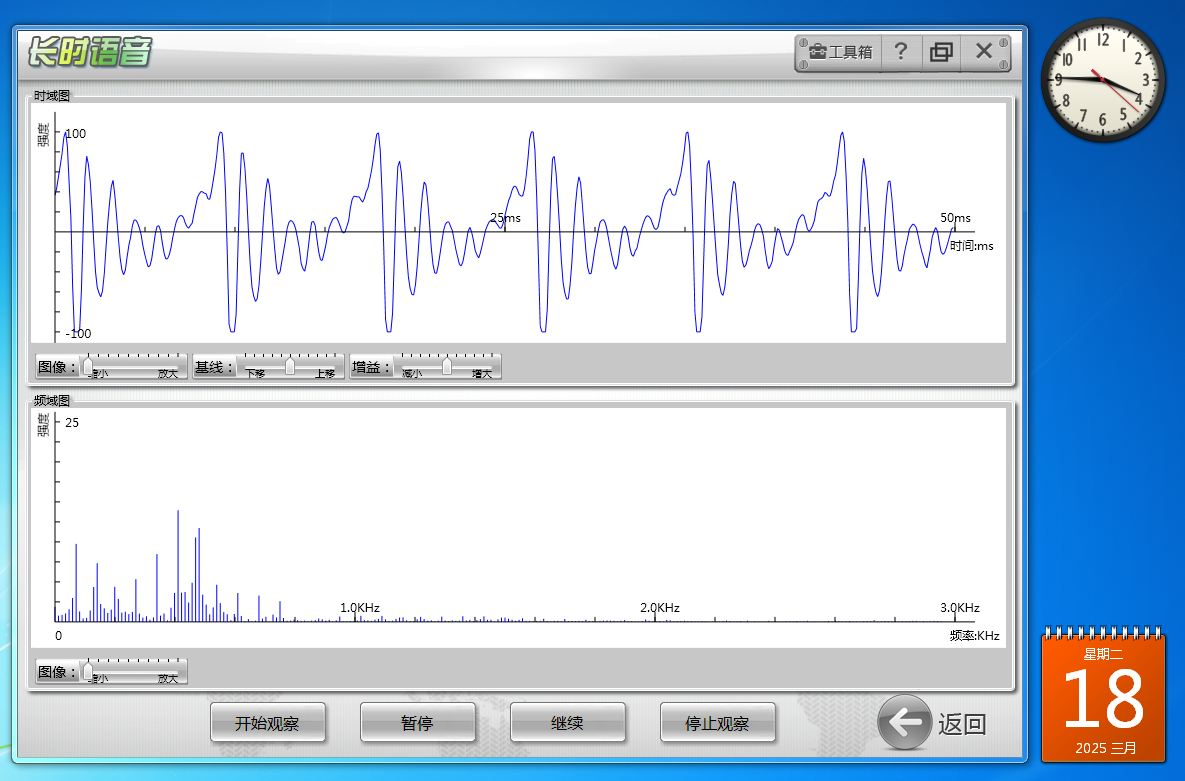
\includegraphics[width=15cm]{Fig/图14 长时语音.JPG}
            \caption{长时语音}
        \end{figure}
    \end{enumerate}

    \item 图像信号的傅里叶分析
    
    用傅里叶分析仪软件提供的“图片分析”模块,分别选择图片“双缝”、“彩色十字”、“光字”以及“箭头”进行空域的傅里叶频谱分析。分别选择低通和高通滤波器进行滤波,记录所用滤波器的参数并将滤波后的图片导出保存。

    \begin{figure}[H]
        \centering
        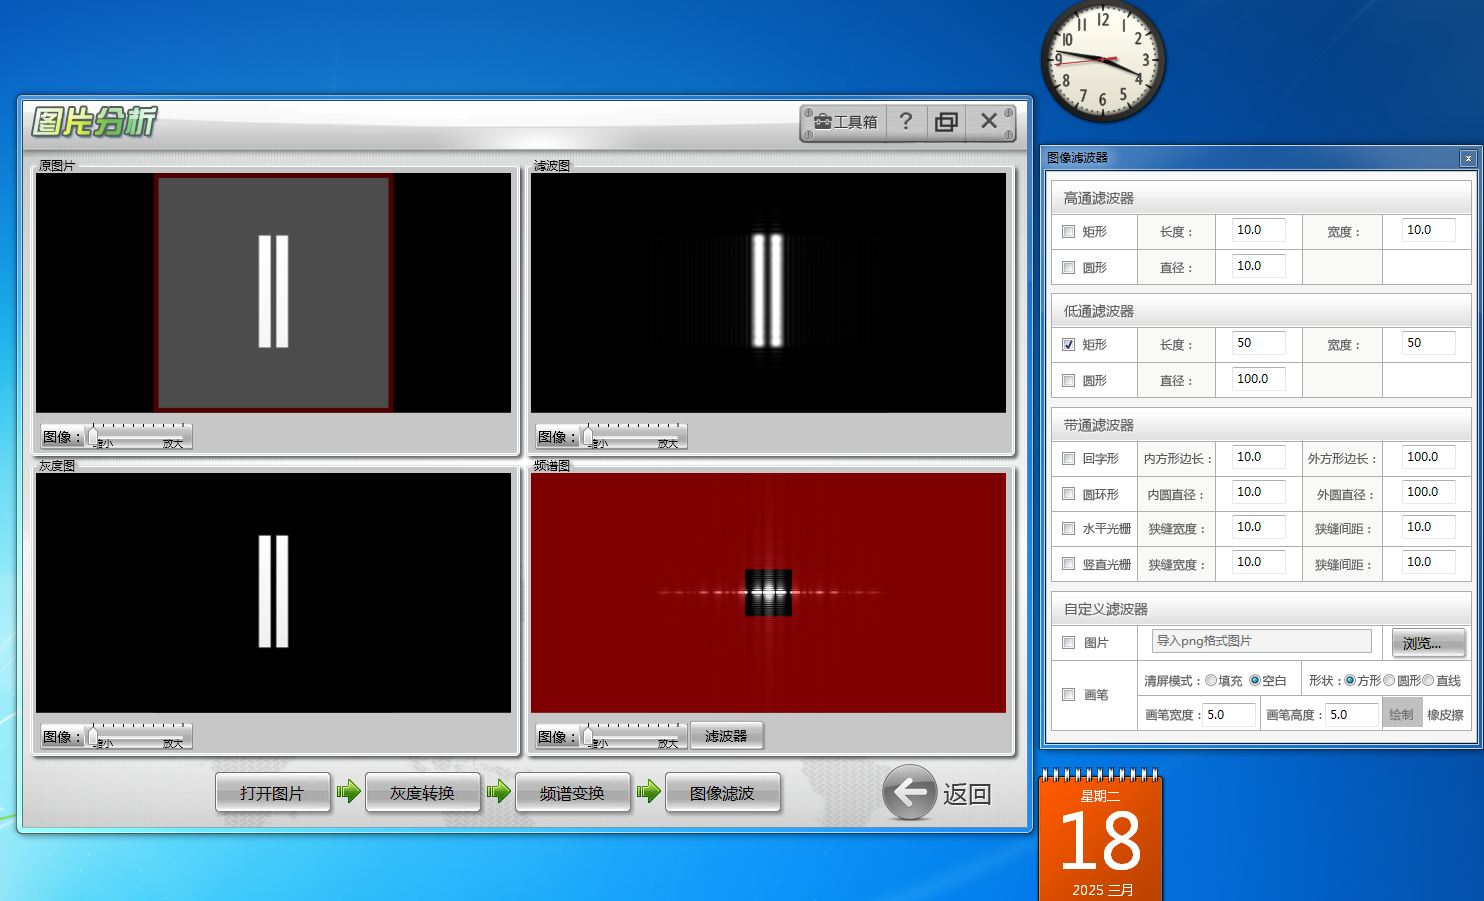
\includegraphics[width=15cm]{Fig/图15 双缝图片低通滤波.JPG}
        \caption{双缝图片低通滤波}
    \end{figure}
    \begin{figure}[H]
        \centering
        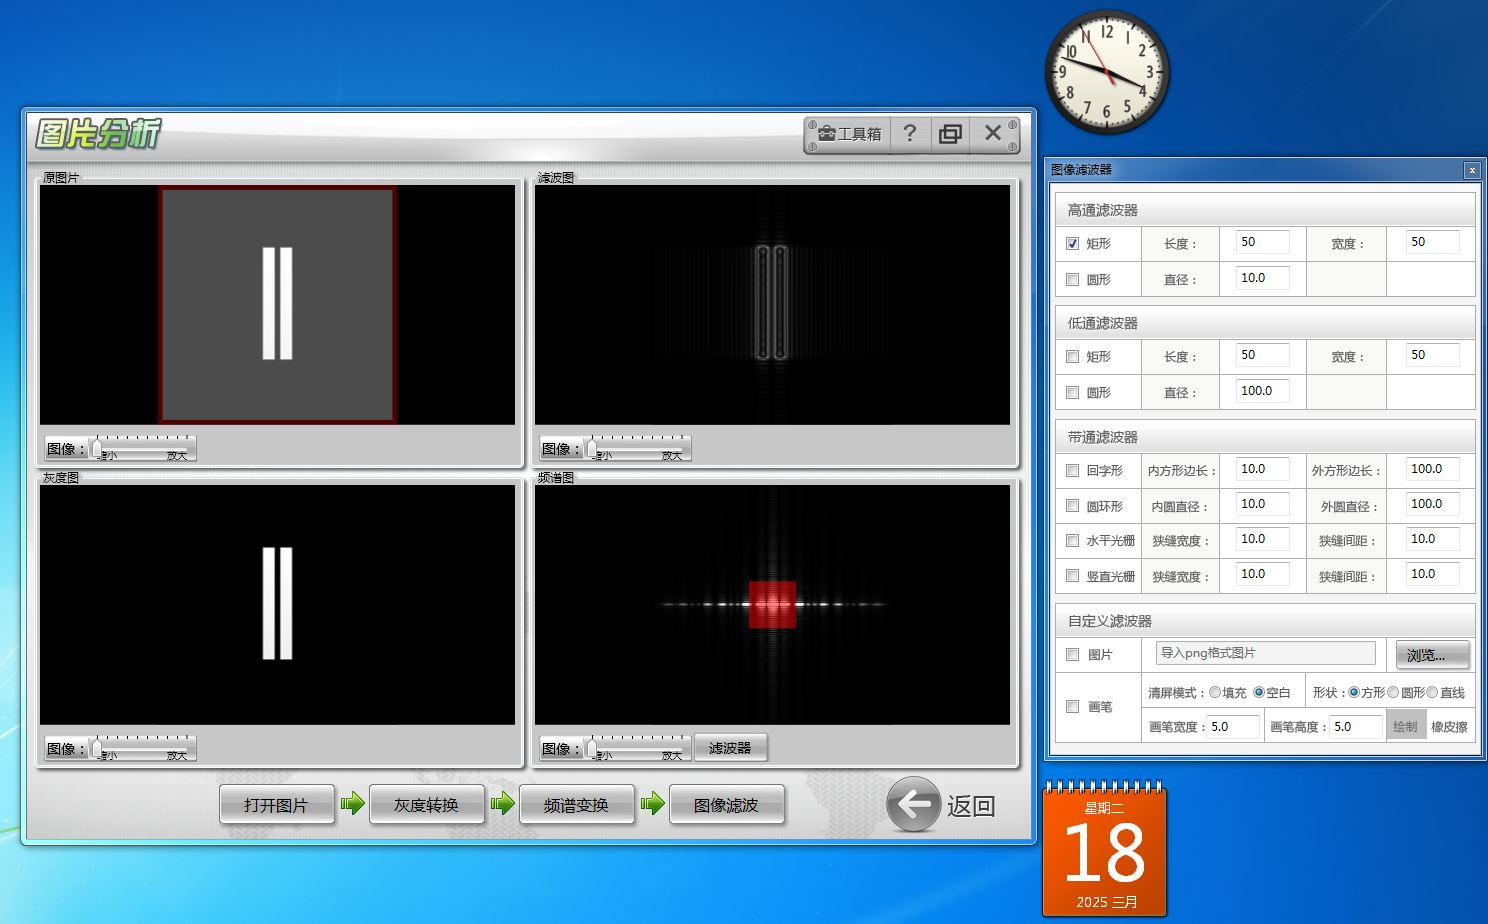
\includegraphics[width=15cm]{Fig/图16 双缝图片高通滤波.JPG}
        \caption{双缝图片高通滤波}
    \end{figure}

    \begin{figure}[H]
        \centering
        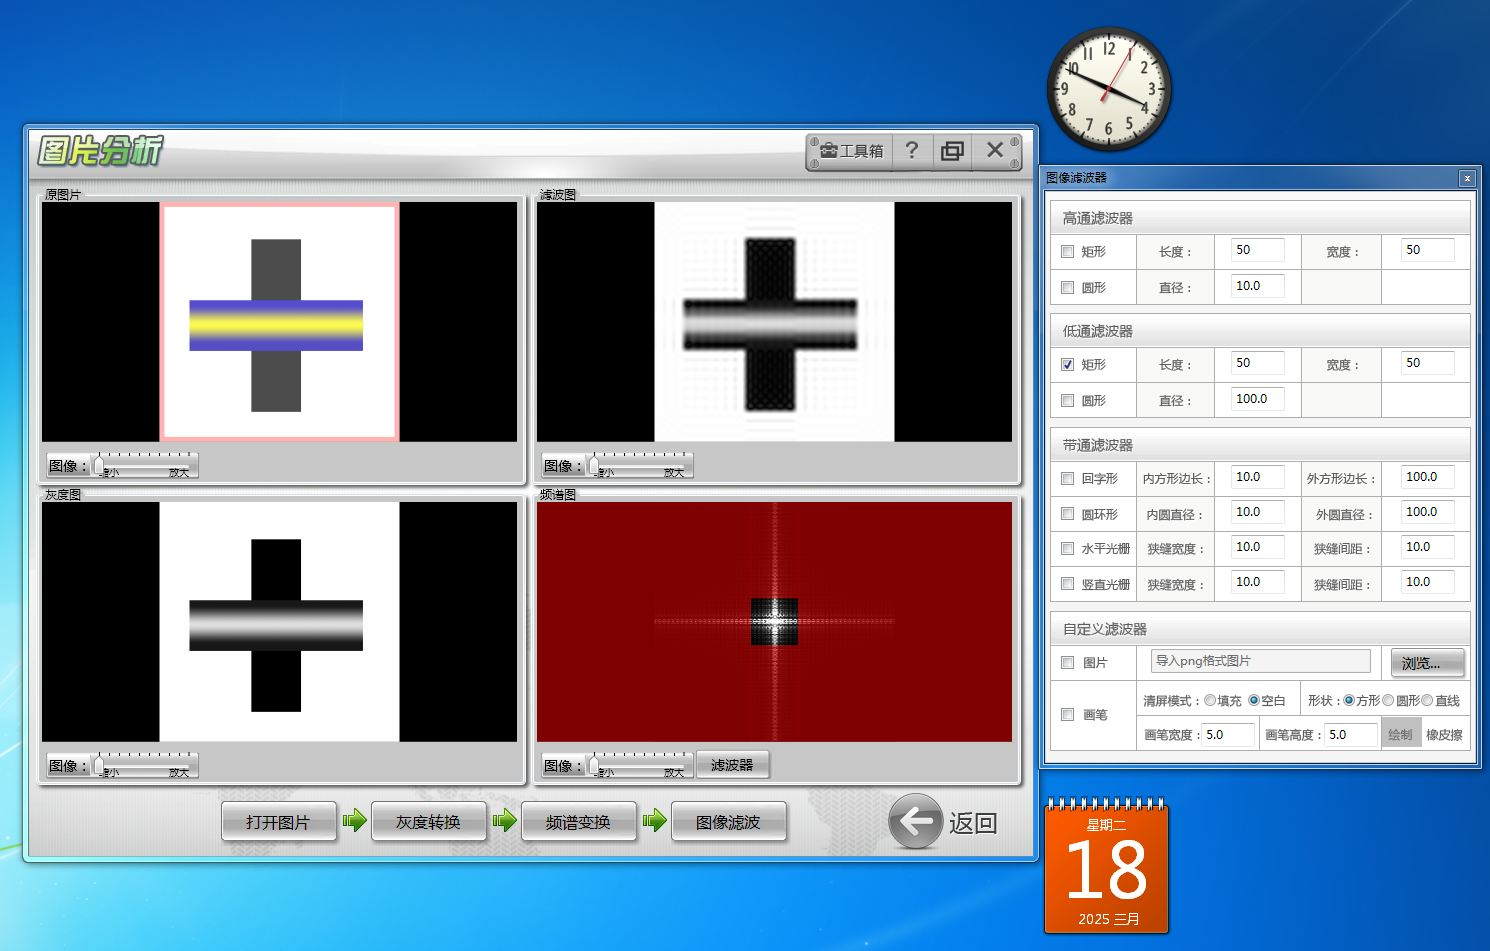
\includegraphics[width=15cm]{Fig/图17 彩色十字图片低通滤波.JPG}
        \caption{彩色十字图片低通滤波}
    \end{figure}
    \begin{figure}[H]
        \centering
        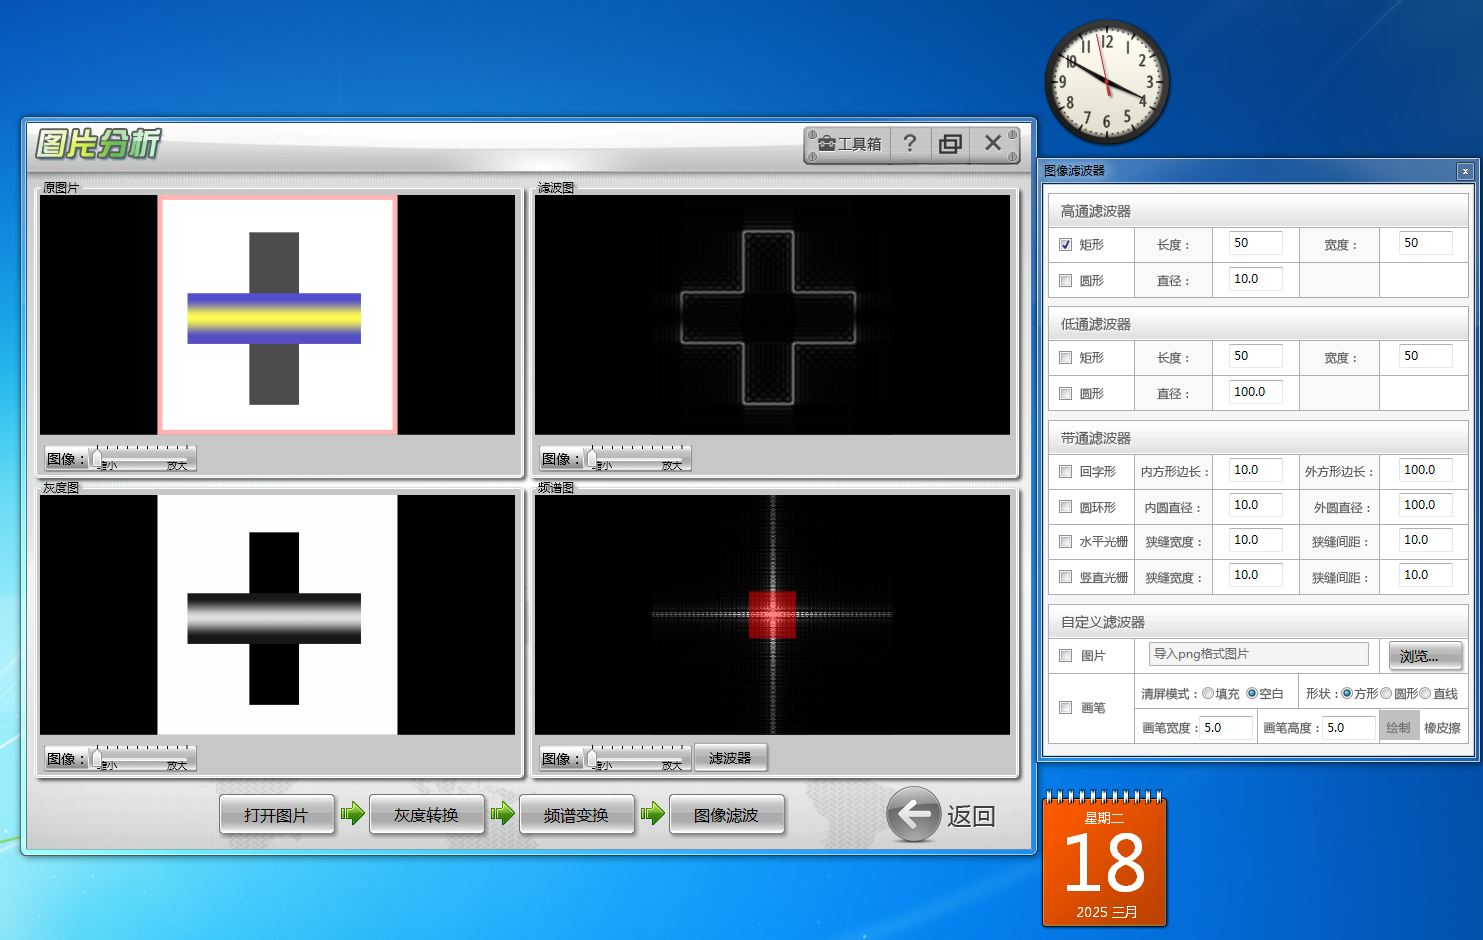
\includegraphics[width=15cm]{Fig/图18 彩色十字图片高通滤波.JPG}
        \caption{彩色十字图片高通滤波}
    \end{figure}

    \begin{figure}[H]
        \centering
        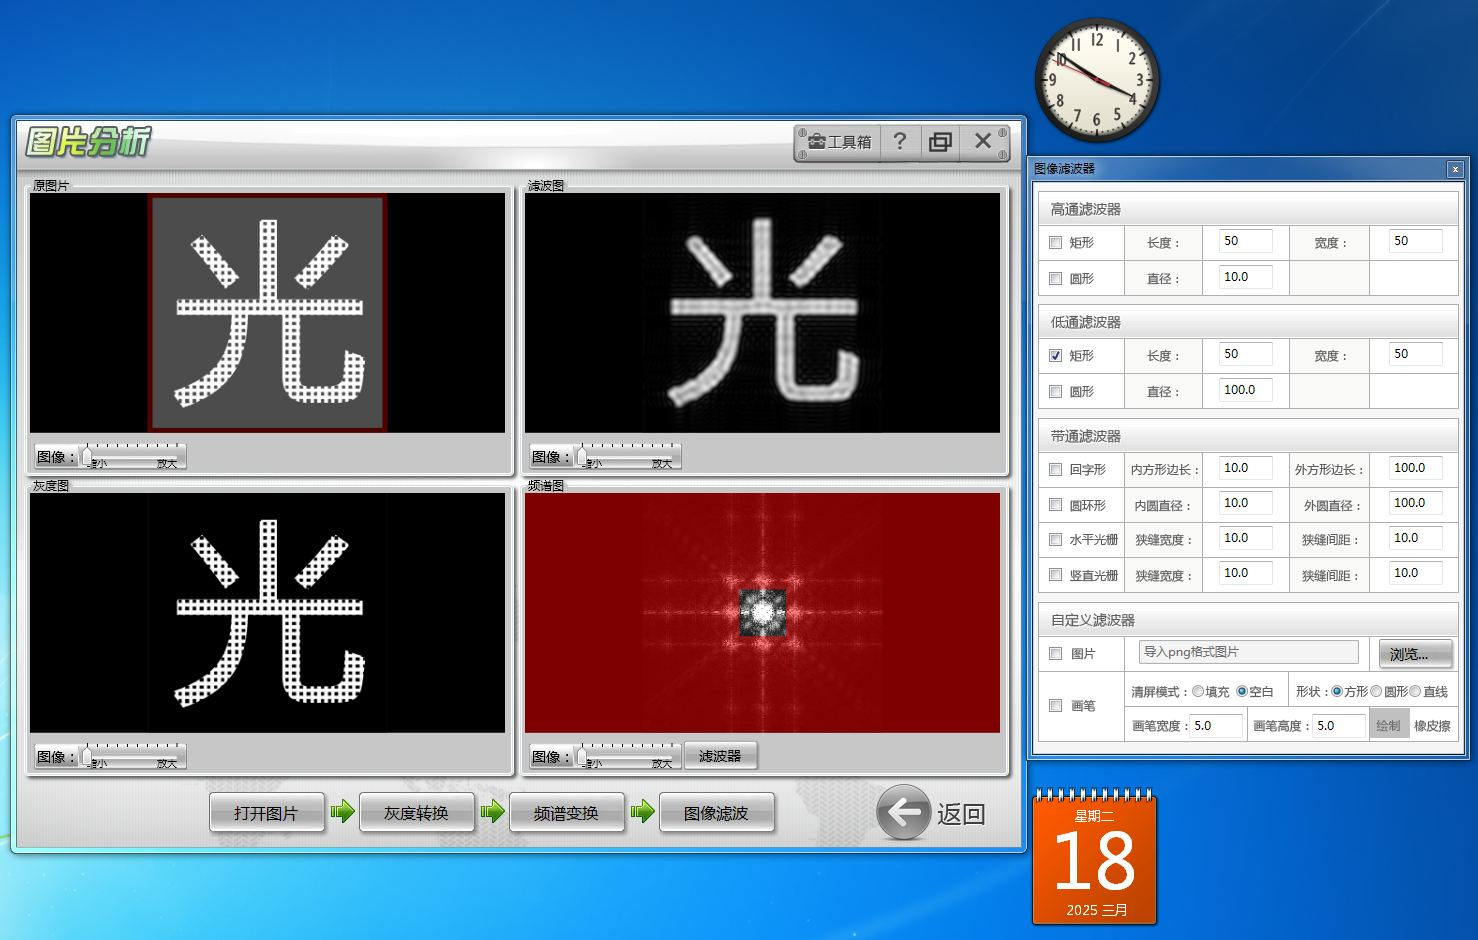
\includegraphics[width=15cm]{Fig/图19 光字图片低通滤波.JPG}
        \caption{光字图片低通滤波}
    \end{figure}
    \begin{figure}[H]
        \centering
        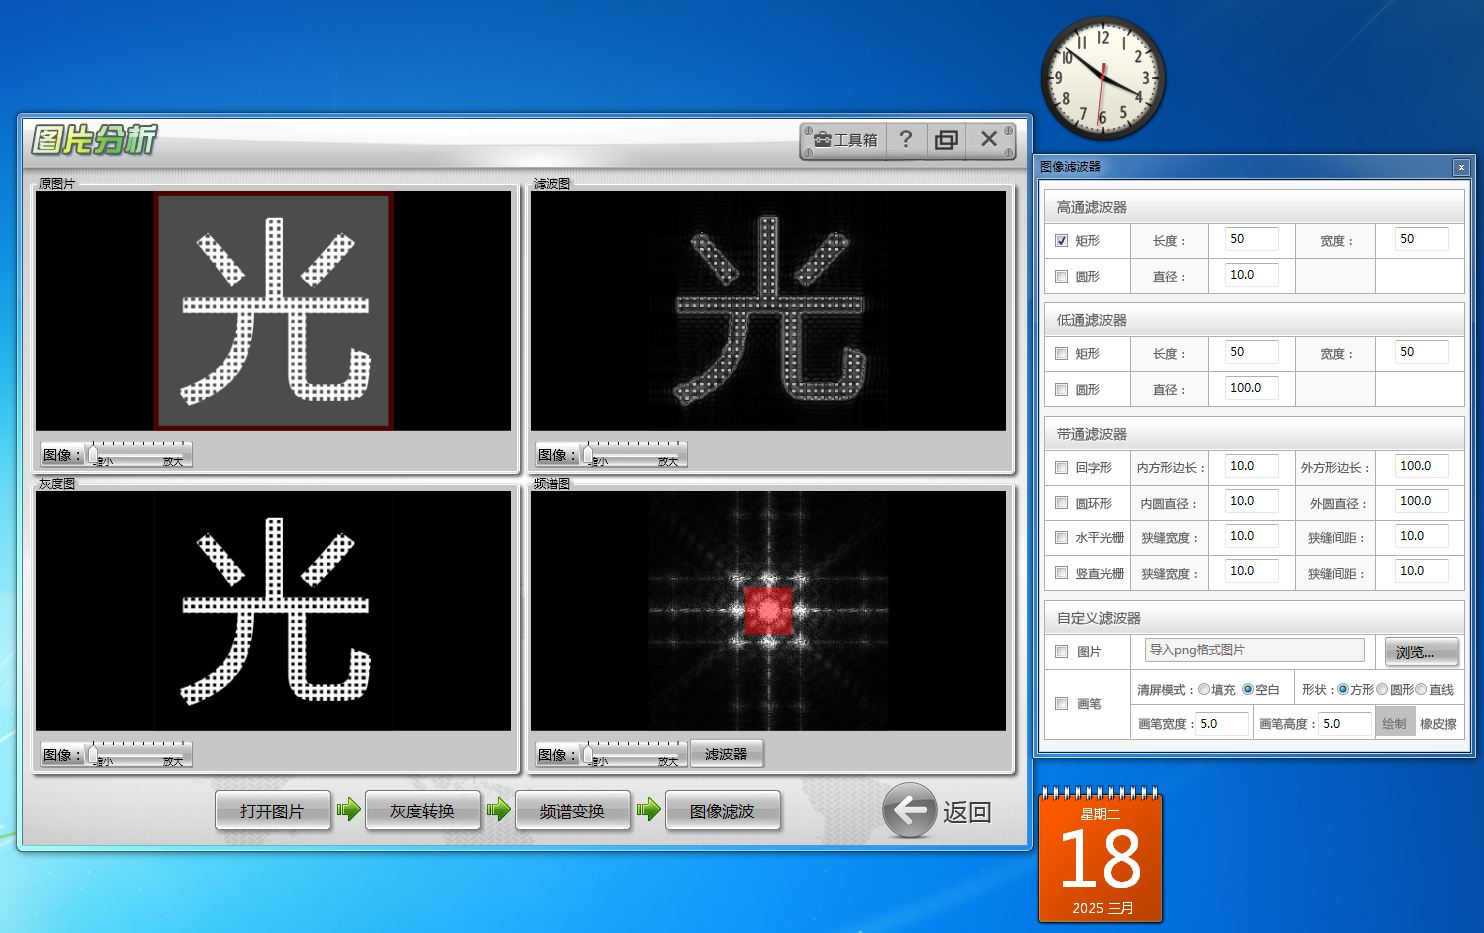
\includegraphics[width=15cm]{Fig/图20 光字图片高通滤波.JPG}
        \caption{光字图片高通滤波}
    \end{figure}

    \begin{figure}[H]
        \centering
        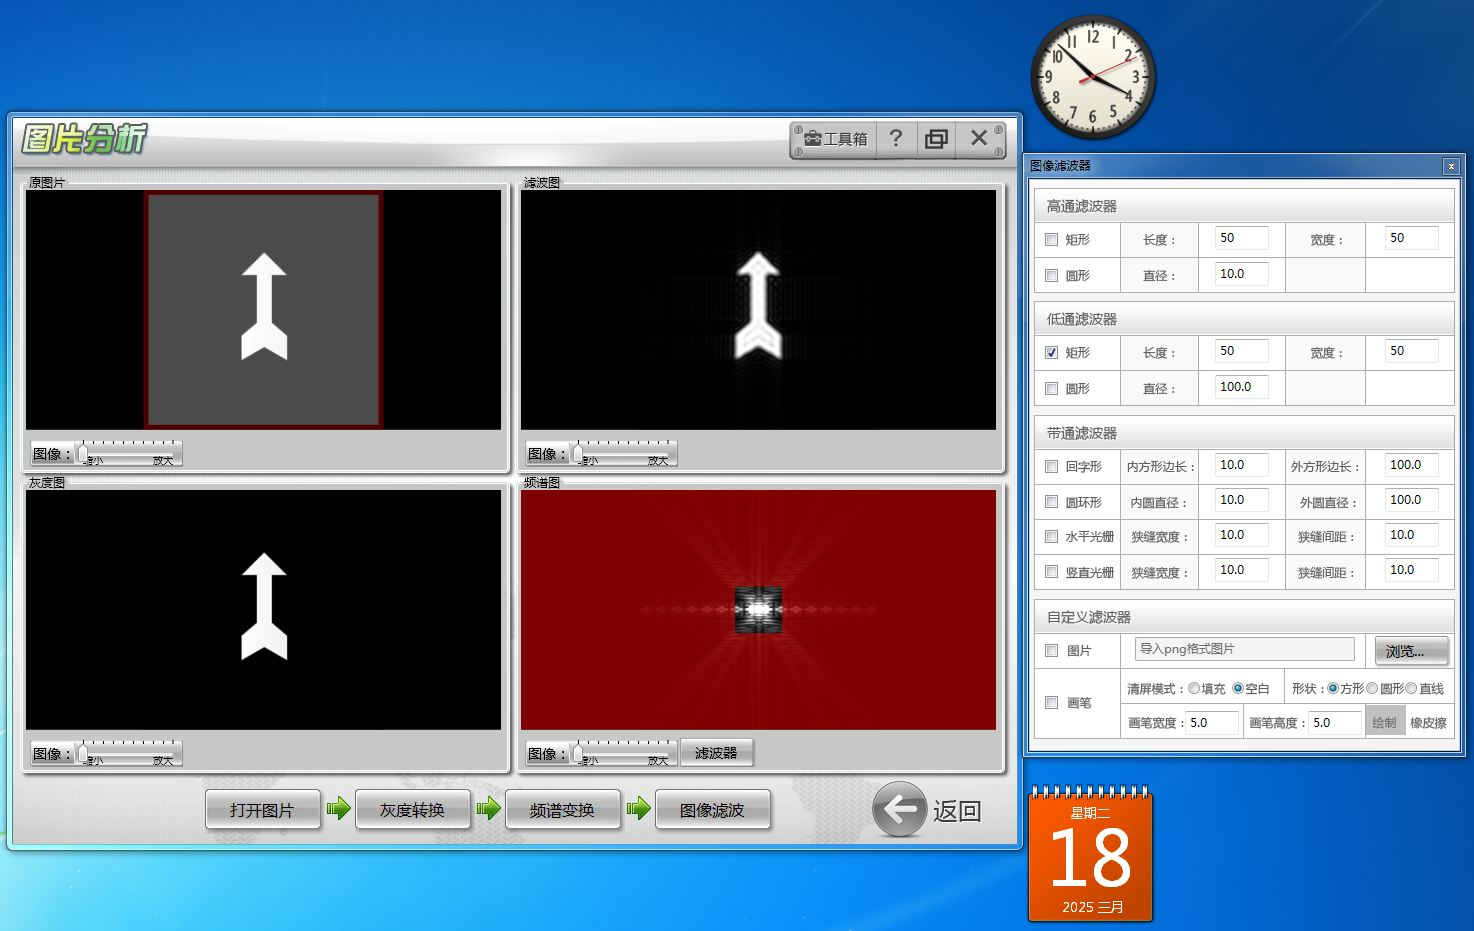
\includegraphics[width=15cm]{Fig/图21 箭头图片低通滤波.JPG}
        \caption{箭头图片低通滤波}
    \end{figure}
    \begin{figure}[H]
        \centering
        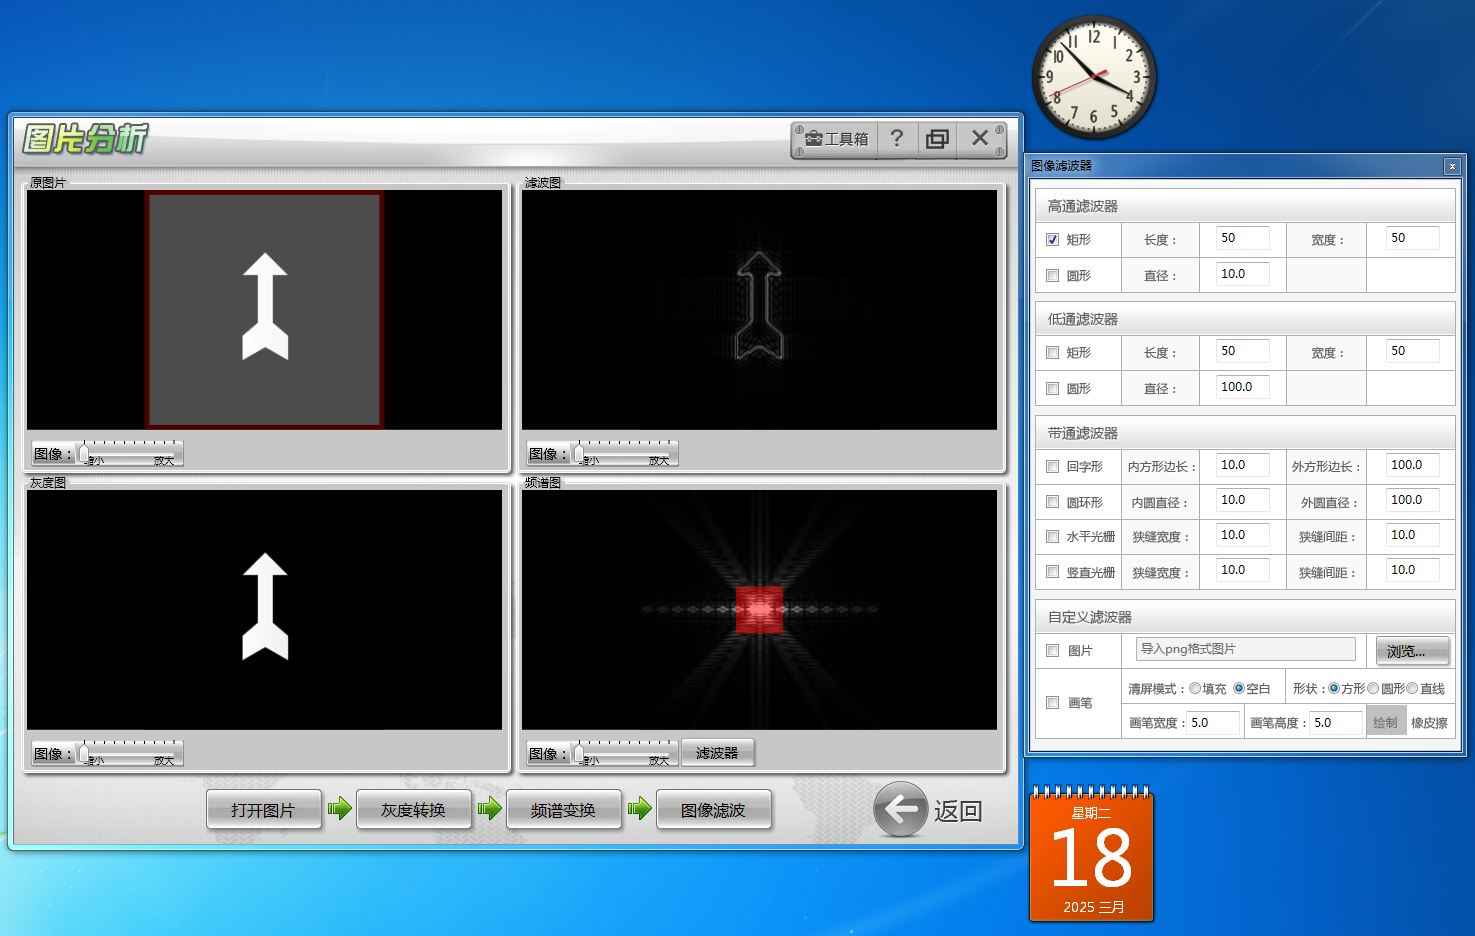
\includegraphics[width=15cm]{Fig/图22 箭头图片高通滤波.JPG}
        \caption{箭头图片高通滤波}
    \end{figure}

\end{enumerate}

\section*{五、数据记录}

对照所有实验内容。每一小项都应有相应截图对应。

\section*{六、数据处理}

\begin{enumerate}
    \item 比较图1和图2,列举差异之处,并分析原因和指出减小差异的方法。
    
    加法器合成的波形相对于方波在波的强度较高时存在波动。原因:图1仅仅由三个较低的不同频率正弦波叠加而成的复合波形,忽略了较高频率的正弦波的影响。可通过选取更多不同的高频率正弦波去消除这个差异。

    \item 比较图3和图4,列举差异之处,并分析原因和指出减小差异的方法。
    
    加法器合成的波形相对于三角波更为圆润,即波峰和波谷处变化不锐利。原因:图3是仅由几个较低的不同频率正弦波叠加而成的复合波形,忽略了较高频率的正弦波的影响。可通过选取更多不同的高频率正弦波去消除这个差异。

    \item 比较图5中“相对强度”栏,指出实验频谱特征与理论预测的异同,并分析原因,比较图2和图5“相对强度”栏中,频率和幅值的比例关系。
    
    实验频谱特征与理论预测频率相似,但是不完全吻合。原因:由于实验仪器和测量误差等因素,可能会导致实验结果与理论预测存在一些差异。频率的比例关系基本符合$1:3:5:\cdots$,幅值的比例关系基本符合$1:\dfrac{1}{3}:\dfrac{1}{5}:\cdots$。

    \item 比较图5中“时域图”和低通滤波“合成图”,列举异同,并分析原因。
    
    合成图大致符合时域图的方波,但在波的强度较高时存在大幅波动。原因:图5是仅由几个较低的不同频率正弦波叠加而成的复合波形,忽略了较高频率的正弦波的影响,可以反映整体样貌但忽略了高频细节。

    \item 比较图6中“时域图”和高通滤波“合成图”,列举异同,并分析原因。
    
    时域图与合成图的周期大致相同,但波形以及波幅差异较大,合成图的图像很尖锐,并且幅度较小。原因:图6是仅由几个较高的不同频率正弦波叠加而成的复合波形,忽略了较低频率的正弦波的影响,只能反应时域图的高频细节而无法反应整体。

    \item 比较图7中“相对强度”栏,指出实验频谱特征与理论预测的异同,并分析原因,比较图4和图7“相对强度”栏中,频率和幅值的比例关系。
    
    实验频谱特征与理论预测频率相似,但是不完全吻合。原因:由于实验仪器和测量误差等因素,可能会导致实验结果与理论预测存在一些差异。频率的比例关系基本符合$1:3:5:\cdots$,幅值的比例关系基本符合$1:\dfrac{1}{3^2}:\dfrac{1}{5^2}:\cdots$。

    \item 比较图7中“时域图”和低通滤波“合成图”,列举异同,并分析原因。
    
    合成图大致符合时域图的三角波,但在波的强度较高时,较为圆滑。原因:图7是仅由几个较低的不同频率正弦波叠加而成的复合波形,忽略了较高频率的正弦波的影响,只能反应时域图的高频细节而无法反应整体,因此波形较为圆滑。

    \item 比较图8中“时域图”和高通滤波“合成图”,列举异同,并分析原因。
    
    时域图与合成图的周期大致相同,但波形以及波幅差异较大,合成图的图像杂乱且幅度很小。原因:图8是仅由几个较高的不同频率正弦波叠加而成的复合波形,忽略了较低频率的正弦波的影响,只能反应时域图的高频细节而无法反应整体。

    \item 记录中心频率$f_1$和$f_2$,比较两次中心频率的变化。
    
    $f_1=1.6\,Hz\;f_2=1.2\,Hz$,深呼吸后,中心频率变小。

    \item 比较“原图片”和“低通滤波图”,列举异同并分析原因。
    
    低通滤波图保留了原图片的大部分细节,但较为模糊。原因:高频代表图像中灰度变化剧烈的点,一般是图像黑白交接处、轮廓或者是噪声。低频代表图像中平滑的,灰度变化不大的点,涵盖了图像中的大部分区域。低通滤波可以让图像变得光滑,滤除图像中的噪点,但丢失了高频的边缘,影响了图像的清晰度。

    \item 比较“原图片”和“高通滤波图”,列举异同并分析原因。
    
    高通滤波图仅保留了原图中的轮廓,相比原图丧失了很大一部分信息。原因:高频代表图像中灰度变化剧烈的点,一般是图像黑白交接处、轮廓或者是噪声。低频代表图像中平滑的,灰度变化不大的点,涵盖了图像中的大部分区域。高通滤波可以检测图像中尖锐、变化明显的地方,但忽略了像素变换缓的区域。
\end{enumerate}

\section*{七、误差分析}

\begin{enumerate}
    \item 频谱分析中,傅里叶分析仪内部电路可能产生干扰波使得波形受到干扰,手工选取周期不完全精确,肯定会有多选和少选,并且仪器精度有限,可能产生误差,从而导致合成波存在误差。
    \item 脉搏实验中,人体脉搏本身不是精准并重复的,并且测量的位置、测试者当时的心理状态,手部的摆放姿势等都会影响信号采集和正常识别。
    \item 语音识别中,周围的环境噪声、录音设备的性能、发声的音量、仪器的误差等都会影响语音采集的质量,并且人每次发音不会完全一致,干扰正常的识别。
\end{enumerate}

\section*{八、实验结论}

实验通过对波形、声音、图像等信号的采集、傅里叶分析、频谱变换、选频、合成,得到如下结论:

傅里叶级数对于具有周期性的波具有极为广泛的适用性,利用不同的方法可以从周期信号中分解出它的各级谐波的频率、幅值和相位。也可根据信号的傅里叶级数表达式,将各级谐波按表达式的要求叠加得到所期望的信号。低频波能体现波形大体结构,高频波则体现波的细节。脉搏、语音信号的分解中能覆盖基频的整数倍频率的波。图像的低通滤波图呈现模糊图像,高通滤波呈现图像轮廓与灰度变化剧烈的点。实验结果与傅里叶原理相符。

\end{document}